\chapter{General problem description}

Indoor tracking is a very complex matter because the common GPS system is unavailable due to the fact that satellite signals are often absent or very imprecise inside buildings.
From that very fact came the need to research other resources that could provide location.
In fact many research labs and companies are developing solutions based on Wi-Fi signals triangulation although this kind of systems are too imprecise for our purpose due too many facts, such as: signal loss, latency, continuous connect and disconnect from a range of Wi-Fi hotspots in order to measure the signal intensity.
Therefore, a wireless solution will impact the autonomy of the device and the installation of Wi-Fi repetitors might be a burden for the final user.
\newline
A marker, which is basically a symbol, avoids all those problems although it brings another level of complexity by introducing other matters, such as: how to recognize the symbol, how to read the data, quantity of information that can be stored, where it should stand, etc.
There are several computer readable markers available on the market and the team decided to make a comparison between them before choosing one.
In fact, before my arrival, an RFID based solution has been produced and tested with simulation and experiments on the field.
This solution used a carpet of RFID passive tags which contained an id corresponding to a position saved on a local map. Furthermore, whenever the rollator with the RFID reader step upon a tag it recognize the associated id and look for it into it's database in order to know the exact position of the user. However, the results of the above mentioned study aren't ready to be published yet, therefore I can not compare the performance of this method with the QRCodes based one but, the current hardware implementation of an RFID reader doesn't allow any calculation on the trajectory of the walker which is a necessary information for our purpose.
The lack of this knowledge could be mitigated with other external resources although the solution proposed on this thesis already overcome this problem. 




\subsection{QR Code quick generalities}

A QRCode is an image containing an encoded binary matrix of data which looks similar to the one in figure \ref{qr} and it allows the storage of alphanumerical, numerical only, binary and ka

\begin{figure}[hbt]
    \centering
    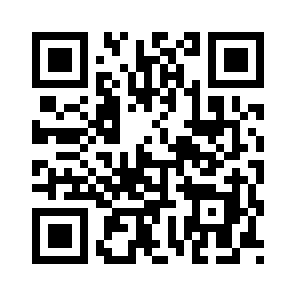
\includegraphics[scale=0.5]{img/qr.png}
    \caption{A generic QrCode}
    \label{qr}
\end{figure}

It is composed by three bigger squares that indicates the position and it might have up to six other smaller squares which helps with the alignment. The basic unit composing the matrix is called module which is the tiniest black are that you can observe. There are 41 versions of it and they differ from each other by an increment of four modules.In fact, every matrix length is fixed and ranges accordingly to the version, from a minimum of 21x21 modules to a maximum of 177x177 modules. The algorithm used to encode offers the opportunity of error correction through the Reed-Solomon technique.\footnote{ according to: \url{http://raidenii.net/files/datasheets/misc/qr_code.pdf}}
Furthermore, because of the above mentioned possibility, there is a need to store codes inside the matrix, the QRcode specification lists four level of error correction: L, M, Q, H which respectively can restore 7, 15, 25 and 30 percent of data according to their codes length.
The QRCode maximum capacity is obtained when using the 40 version combined with an L correction level, this options offers 
In fact, the user, or the program which generates the QRCode for him, has to choose accordingly to the data's size which QRCode version and error correction level to use.

\begin{figure}[hbt]
    \centering
    \caption{Versions of QRCode \protect \footnote{complete table at: \protect \url{http://www.qrcode.com/en/about/version.html}}
    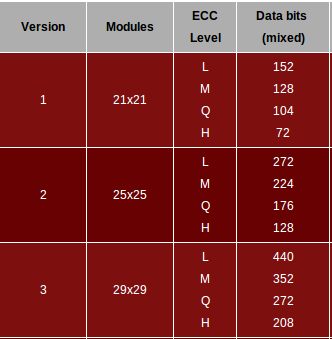
\includegraphics[scale=0.9]{img/qrversion.png}
    \label{qrversion}
\end{figure}


   













  
